
% Aberdeen style guide should be followed when using this
% layout. Their template powerpoint slide is used to extract the
% Aberdeen color and logo but is otherwise ignored (it has little or
% no formatting in it anyway).
%
% http://www.abdn.ac.uk/documents/style-guide.pdf

%%%%%%%%%%%%%%%%%%%% Document Class Settings %%%%%%%%%%%%%%%%%%%%%%%%%
% Pick if you want slides, or draft slides (no animations)
%%%%%%%%%%%%%%%%%%%%%%%%%%%%%%%%%%%%%%%%%%%%%%%%%%%%%%%%%%%%%%%%%%%%%%
%Normal document mode
\documentclass[10pt,compress]{beamer}
%Draft or handout mode
%\documentclass[10pt,compress,handout]{beamer}
%\documentclass[10pt,compress,handout,ignorenonframetext]{beamer}
\usepackage{lmodern}

\usepackage{xcolor}

\newlength{\overwritelength}
\newlength{\minimumoverwritelength}
\setlength{\minimumoverwritelength}{1cm}
\newcommand{\overwrite}[3][red]{%
  \settowidth{\overwritelength}{$#2$}%
  \ifdim\overwritelength<\minimumoverwritelength%
    \setlength{\overwritelength}{\minimumoverwritelength}\fi%
  \stackrel
    {%
      \begin{minipage}{\overwritelength}%
        \color{#1}\centering\small #3\\%
        \rule{1pt}{9pt}%
      \end{minipage}}
    {\colorbox{#1!50}{\color{black}$\displaystyle#2$}}}



%%%%%%%%%%%%%%%%%%%% General Document settings %%%%%%%%%%%%%%%%%%%%%%%
% These settings must be set for each presentation
%%%%%%%%%%%%%%%%%%%%%%%%%%%%%%%%%%%%%%%%%%%%%%%%%%%%%%%%%%%%%%%%%%%%%%
\newcommand{\shortname}{Dr Jeff Gomes}
\newcommand{\fullname}{Dr Jeff Gomes}
\institute{School of Engineering}
\newcommand{\emailaddress}{jefferson.gomes@abdn.ac.uk}
\newcommand{\logoimage}{./FigBanner/UoAHorizBanner}
\title{Advanced Chemical Engineering (EG5597)}
\subtitle{Introduction to Computational Methods for Fluid Dynamics: Partial Differential Equations}
\date[2014-15]{2014-15}



%%%%%%%%%%%%%%%%%%%% Template settings %%%%%%%%%%%%%%%%%%%%%%%%%%%%%%%
% You shouldn't have to change below this line, unless you want to.
%%%%%%%%%%%%%%%%%%%%%%%%%%%%%%%%%%%%%%%%%%%%%%%%%%%%%%%%%%%%%%%%%%%%%%
\usecolortheme{whale}
\useoutertheme{infolines}

% Use the fading effect for items that are covered on the current
% slide.
\beamertemplatetransparentcovered

% We abuse the author command to place all of the slide information on
% the title page.
\author[\shortname]{%
  \fullname\\\ttfamily{\emailaddress}
}


%At the start of every section, put a slide indicating the contents of the current section.
\AtBeginSection[] {
  \begin{frame}
    \frametitle{Section Outline}
    \tableofcontents[currentsection]
  \end{frame}
}

% Allow the inclusion of movies into the Presentation! At present,
% only the Okular program is capable of playing the movies *IN* the
% presentation.
\usepackage{multimedia}
\usepackage{animate}

%% Handsout -- comment out the lines below to create handstout with 4 slides in a page with space for comments
\usepackage{handoutWithNotes}

\mode<handout>
{
\usepackage{pgf,pgfpages}

\pgfpagesdeclarelayout{2 on 1 boxed with notes}
{
\edef\pgfpageoptionheight{\the\paperheight} 
\edef\pgfpageoptionwidth{\the\paperwidth}
\edef\pgfpageoptionborder{0pt}
}
{
\setkeys{pgfpagesuselayoutoption}{landscape}
\pgfpagesphysicalpageoptions
    {%
        logical pages=4,%
        physical height=\pgfpageoptionheight,%
        physical width=\pgfpageoptionwidth,%
        last logical shipout=2%
    } 
\pgfpageslogicalpageoptions{1}
    {%
    border code=\pgfsetlinewidth{1pt}\pgfstroke,%
    scale=1,
    center=\pgfpoint{.25\pgfphysicalwidth}{.75\pgfphysicalheight}%
    }%
\pgfpageslogicalpageoptions{2}
    {%
    border code=\pgfsetlinewidth{1pt}\pgfstroke,%
    scale=1,
    center=\pgfpoint{.25\pgfphysicalwidth}{.25\pgfphysicalheight}%
    }%
\pgfpageslogicalpageoptions{3}
    {%
    border shrink=\pgfpageoptionborder,%
    resized width=.7\pgfphysicalwidth,%
    resized height=.5\pgfphysicalheight,%
    center=\pgfpoint{.75\pgfphysicalwidth}{.29\pgfphysicalheight},%
    copy from=3
    }%
\pgfpageslogicalpageoptions{4}
    {%
    border shrink=\pgfpageoptionborder,%
    resized width=.7\pgfphysicalwidth,%
    resized height=.5\pgfphysicalheight,%
    center=\pgfpoint{.75\pgfphysicalwidth}{.79\pgfphysicalheight},%
    copy from=4
    }%

\AtBeginDocument
    {
    \newbox\notesbox
    \setbox\notesbox=\vbox
        {
            \hsize=\paperwidth
            \vskip-1in\hskip-1in\vbox
            {
                \vskip1cm
                Notes\vskip1cm
                        \hrule width\paperwidth\vskip1cm
                    \hrule width\paperwidth\vskip1cm
                        \hrule width\paperwidth\vskip1cm
                    \hrule width\paperwidth\vskip1cm
                        \hrule width\paperwidth\vskip1cm
                    \hrule width\paperwidth\vskip1cm
                    \hrule width\paperwidth\vskip1cm
                    \hrule width\paperwidth\vskip1cm
                        \hrule width\paperwidth
            }
        }
        \pgfpagesshipoutlogicalpage{3}\copy\notesbox
        \pgfpagesshipoutlogicalpage{4}\copy\notesbox
    }
}
}

%\pgfpagesuselayout{2 on 1 boxed with notes}[letterpaper,border shrink=5mm]
%\pgfpagesuselayout{2 on 1 boxed with notes}[letterpaper,border shrink=5mm]

%%%%% Color settings
\usepackage{color}
%% The background color for code listings (i.e. example programs)
\definecolor{lbcolor}{rgb}{0.9,0.9,0.9}%
\definecolor{UoARed}{rgb}{0.64706, 0.0, 0.12941}
\definecolor{UoALight}{rgb}{0.85, 0.85, 0.85}
\definecolor{UoALighter}{rgb}{0.92, 0.92, 0.92}
\setbeamercolor{structure}{fg=UoARed} % General background and higlight color
\setbeamercolor{frametitle}{bg=black} % General color
\setbeamercolor{frametitle right}{bg=black} % General color
\setbeamercolor{block body}{bg=UoALighter} % For blocks
\setbeamercolor{structure}{bg=UoALight} % For blocks
% Rounded boxes for blocks
\setbeamertemplate{blocks}[rounded]

%%%%% Font settings
% Aberdeen requires the use of Arial in slides. We can use the
% Helvetica font as its widely available like so
% \usepackage{helvet}
% \renewcommand{\familydefault}{\sfdefault}
% But beamer already uses a sans font, so we will stick with that.

% The size of the font used for the code listings.
\newcommand{\goodsize}{\fontsize{6}{7}\selectfont}

% Extra math packages, symbols and colors. If you're using Latex you
% must be using it for formatting the math!
\usepackage{amscd,amssymb} \usepackage{amsfonts}
\usepackage[mathscr]{eucal} \usepackage{mathrsfs}
\usepackage{latexsym} \usepackage{amsmath} \usepackage{bm}
\usepackage{amsthm} \usepackage{textcomp} \usepackage{eurosym}
% This package provides \cancel{a} and \cancelto{a}{b} to "cancel"
% expressions in math.
\usepackage{cancel}

\usepackage{comment} 

% Get rid of font warnings as modern LaTaX installations have scalable
% fonts
\usepackage{type1cm} 

%\usepackage{enumitem} % continuous numbering throughout enumerate commands

% For exact placement of images/text on the cover page
\usepackage[absolute]{textpos}
\setlength{\TPHorizModule}{1mm}%sets the textpos unit
\setlength{\TPVertModule}{\TPHorizModule} 

% Source code formatting package
\usepackage{listings}%
\lstset{ backgroundcolor=\color{lbcolor}, tabsize=4,
  numberstyle=\tiny, rulecolor=, language=C++, basicstyle=\goodsize,
  upquote=true, aboveskip={1.5\baselineskip}, columns=fixed,
  showstringspaces=false, extendedchars=true, breaklines=false,
  prebreak = \raisebox{0ex}[0ex][0ex]{\ensuremath{\hookleftarrow}},
  frame=single, showtabs=false, showspaces=false,
  showstringspaces=false, identifierstyle=\ttfamily,
  keywordstyle=\color[rgb]{0,0,1},
  commentstyle=\color[rgb]{0.133,0.545,0.133},
  stringstyle=\color[rgb]{0.627,0.126,0.941}}

% Allows the inclusion of other PDF's into the final PDF. Great for
% attaching tutorial sheets etc.
\usepackage{pdfpages}
\setbeamercolor{background canvas}{bg=}  

% Remove foot note horizontal rules, they occupy too much space on the slide
\renewcommand{\footnoterule}{}

% Force the driver to fix the colors on PDF's which include mixed
% colorspaces and transparency.
\pdfpageattr {/Group << /S /Transparency /I true /CS /DeviceRGB>>}

% Include a graphics, reserve space for it but
% show it on the next frame.
% Parameters:
% #1 Which slide you want it on
% #2 Previous slides
% #3 Options to \includegraphics (optional)
% #4 Name of graphic
\newcommand{\reserveandshow}[4]{%
\phantom{\includegraphics<#2|handout:0>[#3]{#4}}%
\includegraphics<#1>[#3]{#4}%
}

\newcommand{\frc}{\displaystyle\frac}
\newcommand{\red}{\textcolor{red}}
\newcommand{\blue}{\textcolor{blue}}
\newcommand{\green}{\textcolor{green}}
\newcommand{\purple}{\textcolor{purple}}
 

\begin{document}

% Title page layout
\begin{frame}
  \titlepage
  \vfill%
  \begin{center}
    \includegraphics[clip,width=0.8\textwidth]{\logoimage}
  \end{center}
\end{frame}

% Table of contents
%\frame{ \frametitle{Slides Outline}
%  \tableofcontents
%}


%%%%%%%%%%%%%%%%%%%% The Presentation Proper %%%%%%%%%%%%%%%%%%%%%%%%%
% Fill below this line with \begin{frame} commands! It's best to
% always add the fragile option incase you're going to use the
% verbatim environment.
%%%%%%%%%%%%%%%%%%%%%%%%%%%%%%%%%%%%%%%%%%%%%%%%%%%%%%%%%%%%%%%%%%%%%%




%%%%%%%%%%%%%%%%%%%
%%%   SECTION   %%%
%%%%%%%%%%%%%%%%%%%
\section{Partial Differential Equations (PDE)} 

%##################
%%%   SUBSECTION
%##################
\subsection{Motivation}

%%%
%%% Slide
%%% 
\begin{frame}
 \frametitle{Governing Equations commonly used in Fluid Problems} 
\begin{enumerate}
  \item <1-> The generic form of the conservative (or governing) equations for fluid flow, heat and mass transfers (and for other scalar transport equations) is 
    \visible<2->{
          \begin{equation}
             \frac{\partial}{\partial t}\left(\rho\phi\right) + \nabla\cdot\left(\rho{\bf v}\phi\right) = \nabla\cdot\left(\Gamma\nabla\phi\right) + \mathcal{S}\label{eq:transport}
          \end{equation}}
    \visible<3->{
    with:
    \begin{itemize}
      \item $\phi$: scalar field (e.g., temperature, concentration, etc);
      \item  $\rho$: density;
      \item {\bf v}: velocity vector;
      \item {\it t}: time;
      \item $\Gamma$: diffusion coefficient;
      \item $\mathcal{S}$: source and/or sink term(s);   
      \item $\nabla\cdot\bm{\psi}$: divergent of the vector field $\bm{\psi}$, i.e.,
           \begin{displaymath}  
               \nabla\cdot\bm{\psi} = \frac{\partial \psi_{x}}{\partial x} + \frac{\partial \psi_{y}}{\partial y} + \frac{\partial \psi_{z}}{\partial z}
           \end{displaymath} 
      \item $\nabla\mathcal{F}$: gradient of the scalar  $\mathcal{F}$, i.e., 
           \begin{displaymath} 
               \nabla\mathcal{F} = \frac{\partial \mathcal{F}}{\partial x} \hat{{\bf x}} + \frac{\partial \mathcal{F}}{\partial y} \hat{\bf y} + \frac{\partial \mathcal{F}}{\partial z} \hat{\bf z}
           \end{displaymath} 
      
    \end{itemize}}
\end{enumerate}   
 
\end{frame}


%%%
%%% Slide
%%% 
\begin{frame}
 \frametitle{Governing Equations commonly used in Fluid Problems} 
\begin{enumerate}
  \setcounter{enumi}{1}
  \item <1-> We can rewrite the governing equation (Eqn.~\ref{eq:transport}) to represent the basic conservation quantities, e.g.,
     \begin{enumerate}
        \item <2-> Energy conservation:
           \visible<2->{
           \begin{equation}
              \frac{\partial}{\partial t}\left(\rho h\right) + \nabla\cdot\left(\rho\bm{v}h\right) = \nabla\cdot\left(\kappa\nabla T\right) + \mathcal{S}_{T}
           \end{equation}}
            where $dh=C_{p}dT$ represents the enthalpy and $\kappa$ is the thermal conductivity.
         \item <3-> Momentum conservation:
           \visible<3->{
           \begin{equation}
              \frac{\partial}{\partial t}\left(\rho u\right) + \nabla\cdot\left(\rho\bm{v}u\right) = \nabla\cdot\left(\mu\nabla u\right) - \frac{\partial p}{\partial x} + \mathcal{S}_{u}
           \end{equation}}
          where $p$ and $\mu$ are the pressure and viscosity, respectively.
         \item <4-> Mass conservation of chemical species:
           \visible<4->{
           \begin{equation}
              \frac{\partial}{\partial t}\left(\rho Y_{i}\right) + \nabla\cdot\left(\rho\bm{v}Y_{i}\right) = \nabla\cdot\left(\Gamma_{i}\nabla Y_{i}\right) + \mathcal{R}_{i}
           \end{equation}}
          where $Y_{i}$ and $\Gamma_{i}$ are mass fraction and diffusion coefficient of chemical specie $i$. $\mathcal{R}_{i}$ is the rate of formation of $Y_{i}$ through chemical reactions. 
      \end{enumerate}
\end{enumerate}   
 
\end{frame}


%##################
%%%   SUBSECTION
%##################
\subsection{Classification of PDEs}

%%%
%%%
%%% Slide
%%% 
\begin{frame}
 \frametitle{Order and Linearity}
   \begin{enumerate} 
    %\setcounter{enumi}{2}
      \item<1-> We can generalise a PDE as,
          \visible<1->{
     \begin{equation}
       a\phi_{xx} + b\phi_{xy} + c\phi_{yy} + d\phi_{x} + e\phi_{y} + f = 0\label{Eqn:GenericPDE}
     \end{equation}}
          \visible<2->{
     where {\it a, b, c, d, e, f} and {\it g} are functions of the coordinates $\left(x,y\right)$ but not of $\phi$. And: $\phi_{xx} = \frac{\partial^{2}\phi}{\partial x^{2}}$, $\phi_{xy}=\frac{\partial^{2}\phi}{\partial x\partial y}$ and $\phi_{x}=\frac{\partial \phi}{\partial x}$.}
      \item<3-> The order of a PDE is the {\bf order of the highest occurring derivative}. Equation~\ref{Eqn:GenericPDE} is a \textcolor{blue}{second-order} PDE;
      \item<4-> Many PDEs of physical interest are \textcolor{blue}{first-order in time} and \textcolor{blue}{second-order in space};
      \item<5-> A PDE is called \textcolor{blue}{linear} when none of the functions \textcolor{blue}{\it a-f} depends on $\phi$; 
      \item<6-> Different from ordinary differential equations (ODE), PDEs cannot be classified {\bf only} by the order. This dual classification (i.e., order and linearity) will determine the best (or more appropriate) numerical method to solve the equations.
   \end{enumerate}
\end{frame}

%%%
%%% Slide
%%% 
\begin{frame}
 \frametitle{Hyperbolic, Parabolic and Elliptic PDEs} 
 \begin{enumerate}
   \setcounter{enumi}{5}
   \item <1-> From Eqn.~\ref{Eqn:GenericPDE}, let's define $\mathcal{D}=b^{2}-4ac$. If\footnote{See specific notes from lecture.},
     \begin{enumerate}
        \item <2-> $\mathcal{D}>0$: \textcolor{red}{Hyperbolic PDEs}. In this type of equation, the information travels in certain directions at finite speeds. The problem-solution is considered as a superposition of multiple simple waves. E.g., 1D wave equation and the reduced thermal equation:
          \begin{displaymath}
            u_{tt}-\kappa^{2}u_{xx} = 0, \;\; -\infty\leq x\leq \infty \;\;\text{and}\;\; \left(\rho C_{p}T\right)_{t} + \left(\rho C_{p}\bm{u}T\right)_{x}=0
%\partial_{t}\left(\rho C_{p} T\right) + \partial_{x}\left(\rho C_{p}\bm{u}T\right) = 0
          \end{displaymath} 
        \item <3-> $\mathcal{D}=0$: \textcolor{red}{Parabolic PDEs}. Here, the information travels forward in time, i.e., the solution field can be constructed through a time-step method. E.g., heat equation with constant $\kappa$, $\rho$ and $C_{p}$, with the thermal diffusivity $\alpha=\kappa/\left(\rho C_{p}\right)$:
          \begin{displaymath}
             T_{t} = \alpha T_{xx}
             %\partial_{t}T = \alpha\partial_{xx}T
          \end{displaymath}
        \item <4-> $\mathcal{D}<0$: \textcolor{red}{Elliptic PDEs}. The information is propagated in all directions at infinite speed. It is often used to described steady problems (i.e., in equilibrium). E.g., Poisson and heat conduction equation:
          \begin{displaymath}
             u_{xx} +u_{yy} = 0 \;\;\text{ and } \;\; \nabla\left(\kappa\nabla T\right) = 0
%\partial_{x}\left(\kappa\partial_{x}\right) = 0
          \end{displaymath}
      \end{enumerate}
\end{enumerate}   
 
\end{frame}

%%%
%%% Slide
%%% 
\begin{frame}
 \frametitle{Hyperbolic, Parabolic and Elliptic PDEs} 
 \begin{enumerate}
   \setcounter{enumi}{6}
   \item <1-> Each of the above types can represent distinct physical phenomena and require specific number of boundary/initial conditions;
   \item <2->The solution method to solve each type of PDE is \textcolor{blue}{often specific};
   \item <3-> First-order PDEs,
     \visible<3->{
     \begin{equation}
         d\phi_{x} + e\phi_{y} + f = 0
     \end{equation}
     are \textcolor{blue}{always hyperbolic}.}

 \end{enumerate}   
 
\end{frame}


%%%
%%% Slide
%%% 
\begin{frame}
 \frametitle{Well Posedness of PDE Problems} 
 \begin{enumerate}
   \setcounter{enumi}{9}
   \item <1-> A problem (PDEs + initial and boundary conditions) is considered to be well-posed if it satisfies the following conditions:
      \begin{enumerate}
        \item <2-> a solution exists;
        \item <3-> the solution is unique;
        \item <4-> the solution depends continuously on the data.
      \end{enumerate}
    \item <5-> The property of \textcolor{blue}{well-posedness} is critical to numerically solve set of PDEs. Thus, a numerical method will not work correctly on \textcolor{blue}{ill-posed} problems. 
 \end{enumerate}   
 
\end{frame}


%%%
%%% Slide
%%% 
\begin{frame}
 \frametitle{Boundary Conditions} 
 \begin{enumerate}
   \setcounter{enumi}{11}
   \item <1-> The generic PDE (Eqn.~\ref{Eqn:GenericPDE}),
     \visible<1->{
      \begin{displaymath}
        \mathcal{L}\left(\phi\right) = G\left(x,y\right)\;\;\text{ for }\;\;x,y\in\mathcal{R}
      \end{displaymath}
      where $\mathcal{L}$ is a linear partial differential operator;}
   \item <2-> The boundary conditions associated with this PDE is represented by the {\it boundary operator},
     \visible<2->{
      \begin{equation}
        \mathcal{B}\left(\phi\right) = f\left(x,y\right)\;\;\text{ for }\;\;x,y\in\mathcal\partial{R}
      \end{equation}
      where $\partial\mathcal{R}$ represents the boundary of the region $\mathcal{R}$ and $f(x,y)$ is a given function of $x$ and $y$.}

  
 \end{enumerate}   
 
\end{frame}


%%%
%%% Slide
%%% 
\begin{frame}
 \frametitle{Boundary Conditions} 
 \begin{enumerate}
   \setcounter{enumi}{13}   
   \item <1-> Boundary conditions can be divided into 3 types: \textcolor{blue}{Dirichlet}, \textcolor{blue}{Neumann} and \textcolor{blue}{Robin};
      \begin{enumerate}
          \item <2-> \textcolor{blue}{Dirichlet BC}: if $\mathcal{B}\left(\phi\right)=\phi$, the boundary conditions is represented by the dependent variable specified on the boundary $\partial\mathcal{R}$; e.g., a prescribed wall temperature is defined as $T\left(x=0,t\right)=T_{\text{wall}}$;
          \item <3-> \textcolor{blue}{Neumann BC}: if $\mathcal{B}\left(\phi\right) = \frac{\partial\phi}{\partial n}=\nabla\phi\cdot\hat{n}$, the boundary conditions is represented by a specified normal derivative at each point in the boundary, e.g., imposed thermal flux across the wall;
          \item <4-> \textcolor{blue}{Robin BC}: here the {\it boundary operator} is a {\it linear combination} of Dirichlet and Neumann boundary conditions, i.e., $\mathcal{B}\left(\phi\right)=\alpha\frac{\partial\phi}{\partial n}+ \beta\phi$ (where $\alpha$ and $\beta$ are constants).
      \end{enumerate} 
   \item <5->   The 1D heat equation,
     \visible<5->{
        \begin{displaymath}
          \alpha\frac{\partial^{2}T}{\partial x^{2}} = \frac{\partial T}{\partial t} 
        \end{displaymath}
        $\alpha = \kappa/\left(\rho C_{p}\right)$ is the thermal diffusivity, where $\rho$ (density), $C_{p}$ (heat capacity) and $\kappa$ (heat conductivity) are constants.}
 \end{enumerate}   
 
\end{frame}


%%%
%%% Slide
%%% 
\begin{frame}
 \frametitle{Boundary Conditions} 
 \begin{enumerate}
   \setcounter{enumi}{15}     
   \item <1-> Then for the heat equation, 
      \begin{enumerate}
        \item <2-> Dirichlet boundary-initial value problem can be represented as,
          \visible<2->{
          \begin{eqnarray}
             \text{PDE:} && \frac{\partial T}{\partial t} - \alpha\frac{\partial^{2}T}{\partial x^{2}} = 0,\;\; t>0,\;\;0<x<L \nonumber \\
             \text{BC:}  && T\left(0,t\right) = T_{0}, \;T\left(L,t\right)=T_{\text{L}} \nonumber \\
             \text{IC:}  && T\left(x,0\right) = f\left(x\right)\nonumber
          \end{eqnarray}} 
        \item <3-> Neumann boundary-initial value problem can be represented as,
          \visible<3->{
          \begin{eqnarray}
             %\text{PDE:} && \frac{\partial T}{\partial t} - \alpha\frac{\partial^{2}T}{\partial x^{2}} = 0,\;\; t>0,\;\;0<x<L \nonumber \\
             \text{BC:}  && - \frac{\partial T\left(0,t\right)}{\partial x}=T_{0},\; \frac{\partial T\left(\text{L},t\right)}{\partial x}=T_{\text{L}} \nonumber \\
             \text{IC:}  && T\left(x,0\right) = f\left(x\right)\nonumber
          \end{eqnarray}} 
        \item <4-> Robin boundary-initial value problem can be represented as,
          \visible<4->{
          \begin{eqnarray}
             %\text{PDE:} && \frac{\partial T}{\partial t} - \alpha\frac{\partial^{2}T}{\partial x^{2}} = 0,\;\; t>0,\;\;0<x<L \nonumber \\
             \text{BC:}  && - \frac{\partial T\left(0,t\right)}{\partial x}+hT\left(0,t\right)=\Psi_{0},\; \frac{\partial T\left(\text{L},t\right)}{\partial x}+hT\left(\text{L},t\right)=\Psi_{\text{L}} \nonumber \\
             \text{IC:}  && T\left(x,0\right) = f\left(x\right)\nonumber
          \end{eqnarray}} 
  
      \end{enumerate}   
 \end{enumerate}   
 
\end{frame}

%##################
%%%   SUBSECTION
%##################
\subsection{Geometric Discretisation}

%%%
%%% Slide
%%% 
\begin{frame}
 \frametitle{Computational Mesh Grid} 
 \begin{enumerate}
   \item <1-> The approximated solution of a (set of) PDE(s) is discretised through the geometric domain represented by a finite number of cells / elements;
   \item <2-> The unknowns in the PDEs are solved at each node and/or element / cell $\Longleftrightarrow$ the number of \textcolor{blue}{degrees of freedom} of a solution field is determined by the number of nodes and/or elements / cells;
   \item <3-> Most commercial / academic CFDs and flow simulators employ (a) structured, (b) block-structured and (c) unstructured mesh grids; 
    \visible<3->{
    \begin{center}
     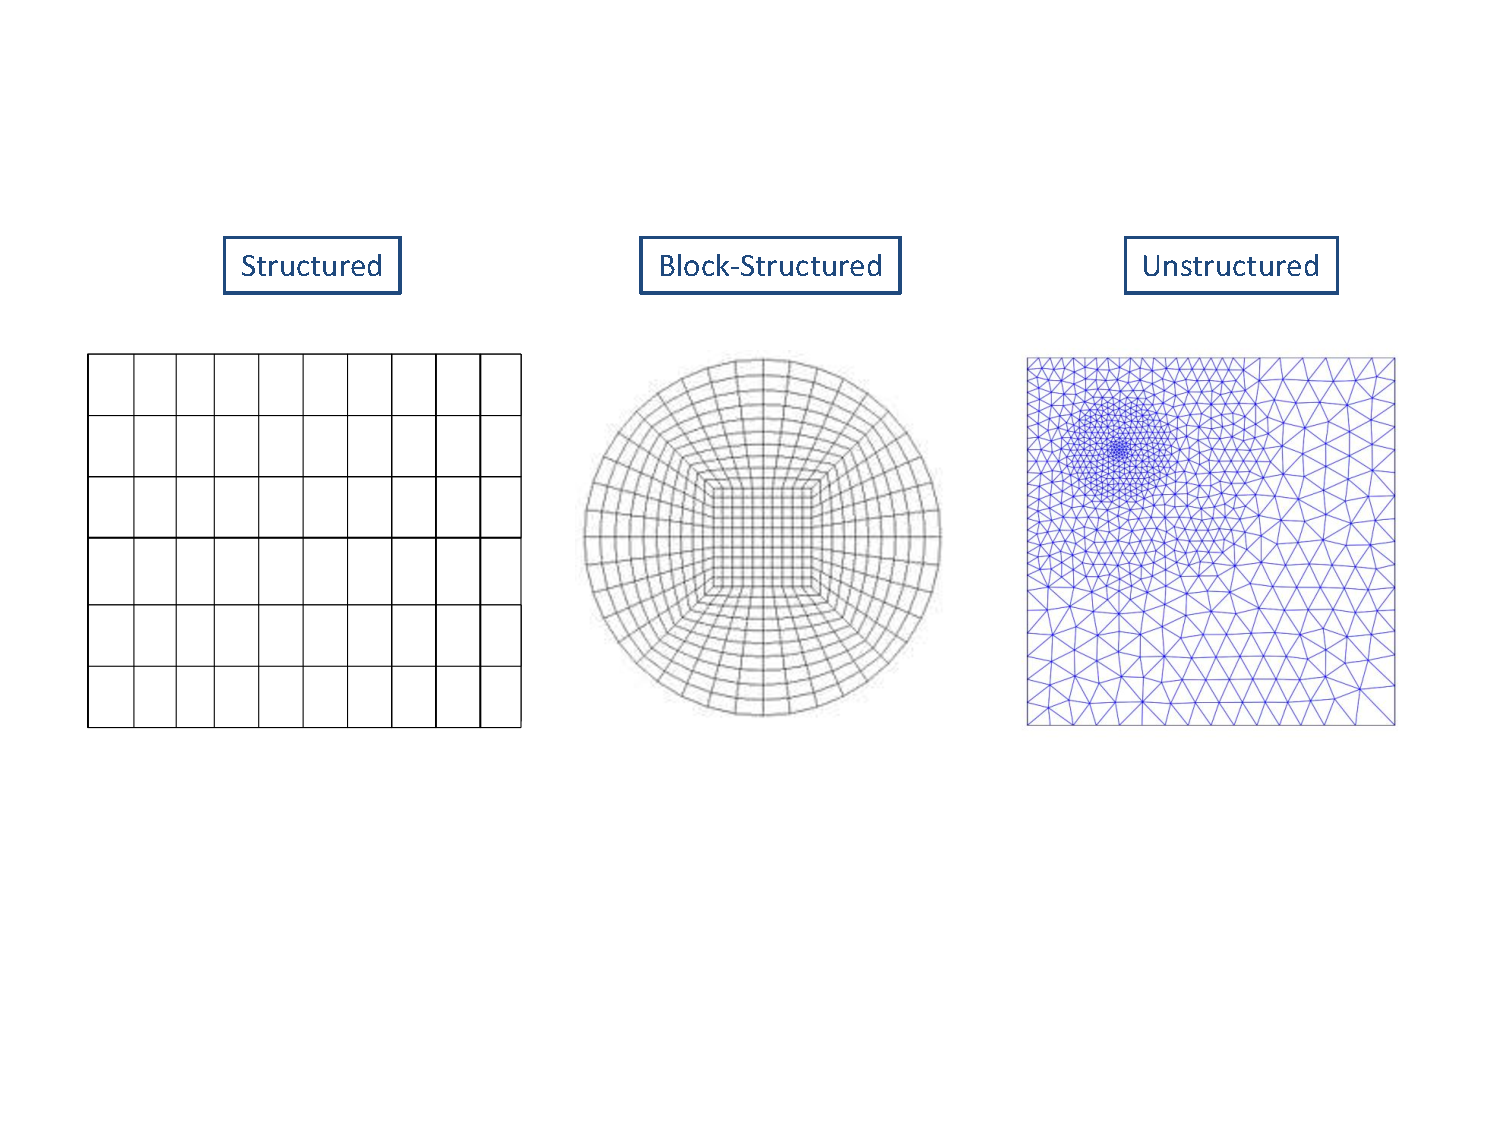
\includegraphics[width=6.5cm, height=2.5cm, clip]{./Figs/MeshGrid_Examples2.pdf}
    \end{center}}
    \item <4-> In \textcolor{blue}{Structured Meshes}:
    \begin{enumerate}
       \item <5-> Grid-lines intersect with a prescribed (and regular) number of grid-lines; 
       \item <6-> Limited to simple geometries and often require local mesh refinement.
    \end{enumerate}  
 \end{enumerate}  

\end{frame}

%%%
%%% Slide
%%% 
\begin{frame}
 \frametitle{Computational Mesh Grid} 
 \begin{enumerate}
   \setcounter{enumi}{4}    
   \item <1-> \textcolor{blue}{Block-Structured Meshes}:
    \begin{enumerate}
       \item <2-> Multi-level subdivision of structured mesh within blocks; 
       \item <3-> Have more flexibility than structured mesh and allow local refinement block-wise;
    \end{enumerate}    
   \item <4-> \textcolor{blue}{Unstructured Meshes}:
    \begin{enumerate}
       \item <5-> Can be used in arbitrary geometries with sensible (adaptive) mesh refinement;
       \item <6-> Consist of triangles or quadrilaterals in 2D and tetrahedra or hexahedra in 3D.
    \end{enumerate}  
    \visible<1->{
    \begin{center}
     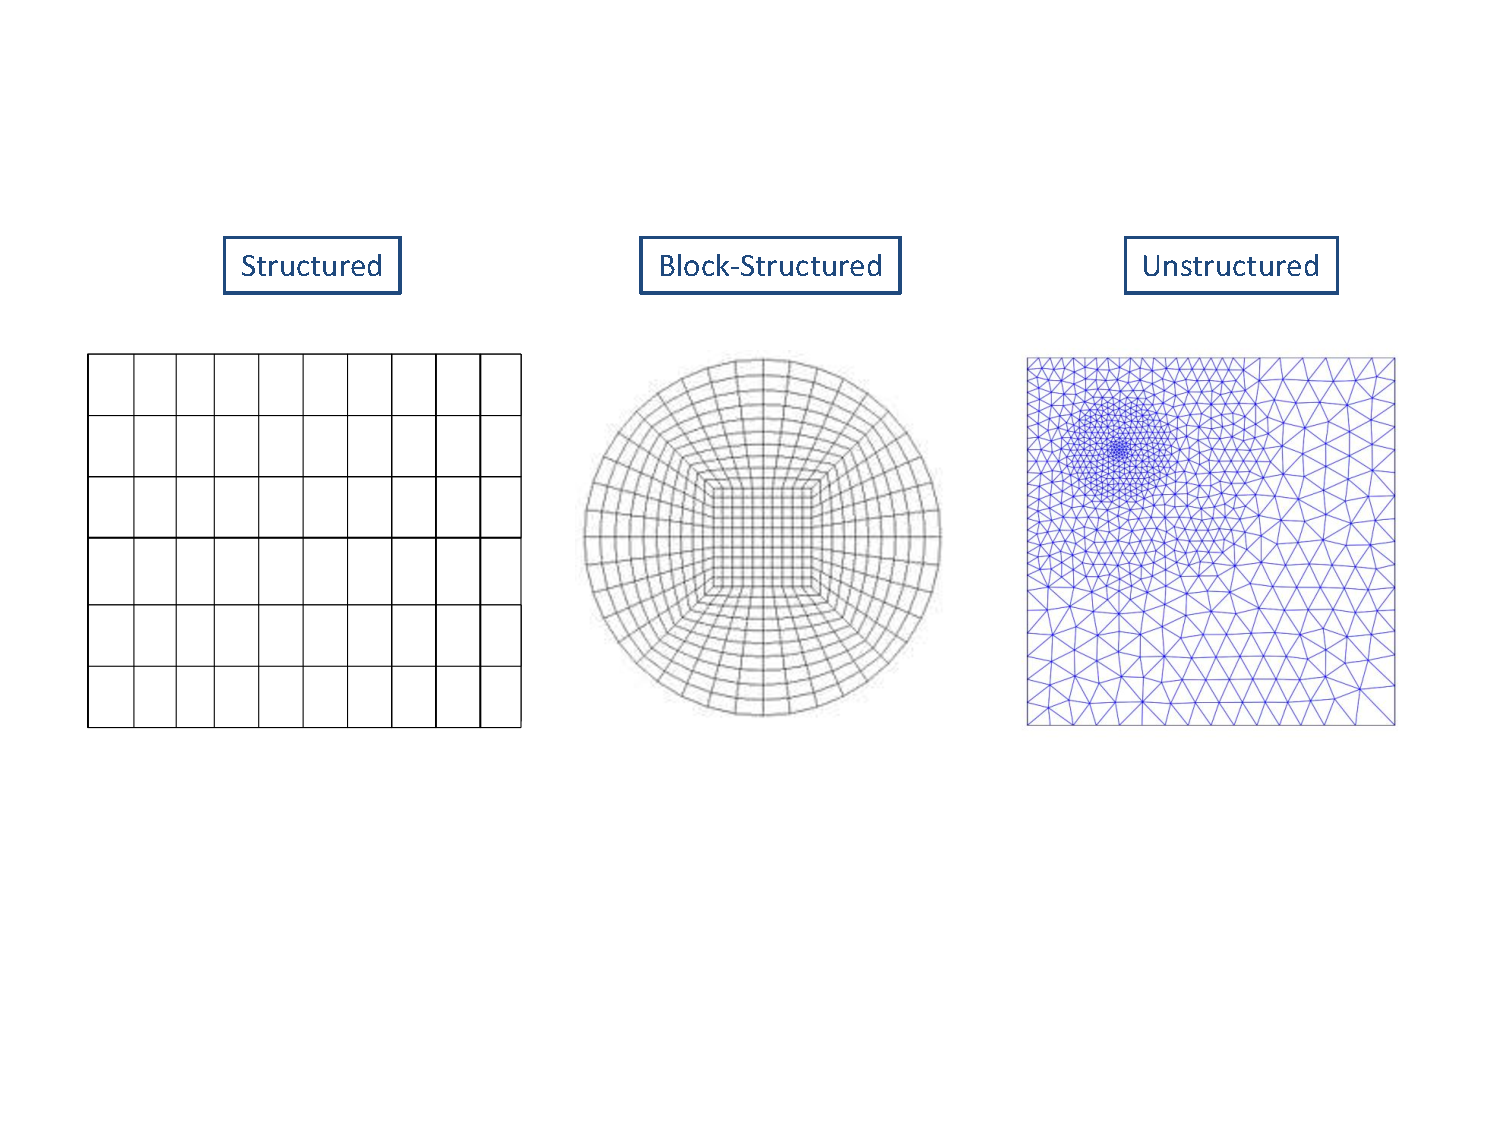
\includegraphics[width=6.5cm, height=2.5cm, clip]{./Figs/MeshGrid_Examples2.pdf}
    \end{center}} 
 \end{enumerate}  

\end{frame}



 
%##################
%%%   SUBSECTION
%##################
\subsection{Spatial Discretisation}

%%%
%%% Slide
%%% 
\begin{frame}
 \frametitle{Finite Difference Method (FDM)} 

\begin{enumerate}
  \item <1-> In the FDM, the derivatives of the governing PDE (Eqn.~\ref{eq:transport}) are approximated using Taylor series expansions truncated at (relativeley) low-order;
  \item <2-> For example, if we consider the 1D transport equation with constant diffusion coefficient and no unsteady or advective terms,
    \visible<2->{
          \begin{equation}
            \textcolor{red}{\cancelto{0}{\frac{\partial}{\partial t}\left(\rho\phi\right)}} + \textcolor{red}{\cancelto{0}{\frac{\partial}{\partial x}\left(\rho\bm{v}\phi\right)}}= \nabla\cdot\left(\Gamma\nabla\phi\right) + \mathcal{S} \Longrightarrow \textcolor{blue}{\Gamma\frac{d^{2}\phi}{dx^{2}} +\mathcal{S} = 0}\label{eq:1Dtransport_simplified}
          \end{equation}}
\end{enumerate}  
 
\end{frame}


%%%
%%% Slide
%%%
\begin{frame}
 \frametitle{Finite Difference Method (FDM)}

  \begin{enumerate}
    \setcounter{enumi}{2}
      \item <2-> The diffusion term can be discretised using the Taylor series expansion:
        \visible<2->{
          \begin{eqnarray}
            \phi_{i-1} = \phi_{i} - \Delta x\left(\frac{d\phi}{d x}\right)_{i} + \frac{\left(\Delta x\right)^{2}}{2}\left(\frac{d^{2}\phi}{dx^{2}}\right)_{i} + \overwrite{\mathcal{O}\left[\left(\Delta x\right)^{3}\right]}{truncation order} \label{Eqn:FDMDisc1}\\ 
            \phi_{i+1} = \phi_{i} + \Delta x\left(\frac{d\phi}{d x}\right)_{i} + \frac{\left(\Delta x\right)^{2}}{2}\left(\frac{d^{2}\phi}{dx^{2}}\right)_{i} + \mathcal{O}\left[\left(\Delta x\right)^{3}\right]\label{Eqn:FDMDisc2}
          \end{eqnarray}}
      \item <3-> If we subtract Eqn.~\ref{Eqn:FDMDisc2} from~\ref{Eqn:FDMDisc1}, and sum them up:
       \visible<3->{
         \begin{displaymath}
            \left(\frac{d\phi}{d x}\right)_{i} = \frac{\phi_{i+1}-\phi_{i-1}}{2\Delta x} \;\;\text{ and }\;\; \left(\frac{d^{2}\phi}{d x^{2}}\right)_{i} = \frac{\phi_{i-1}+\phi_{i+1}-2\phi_{i}}{\left(\Delta x\right)^{2}}
         \end{displaymath}}
  \end{enumerate}  
     \visible<1->{ 
       \begin{center}
         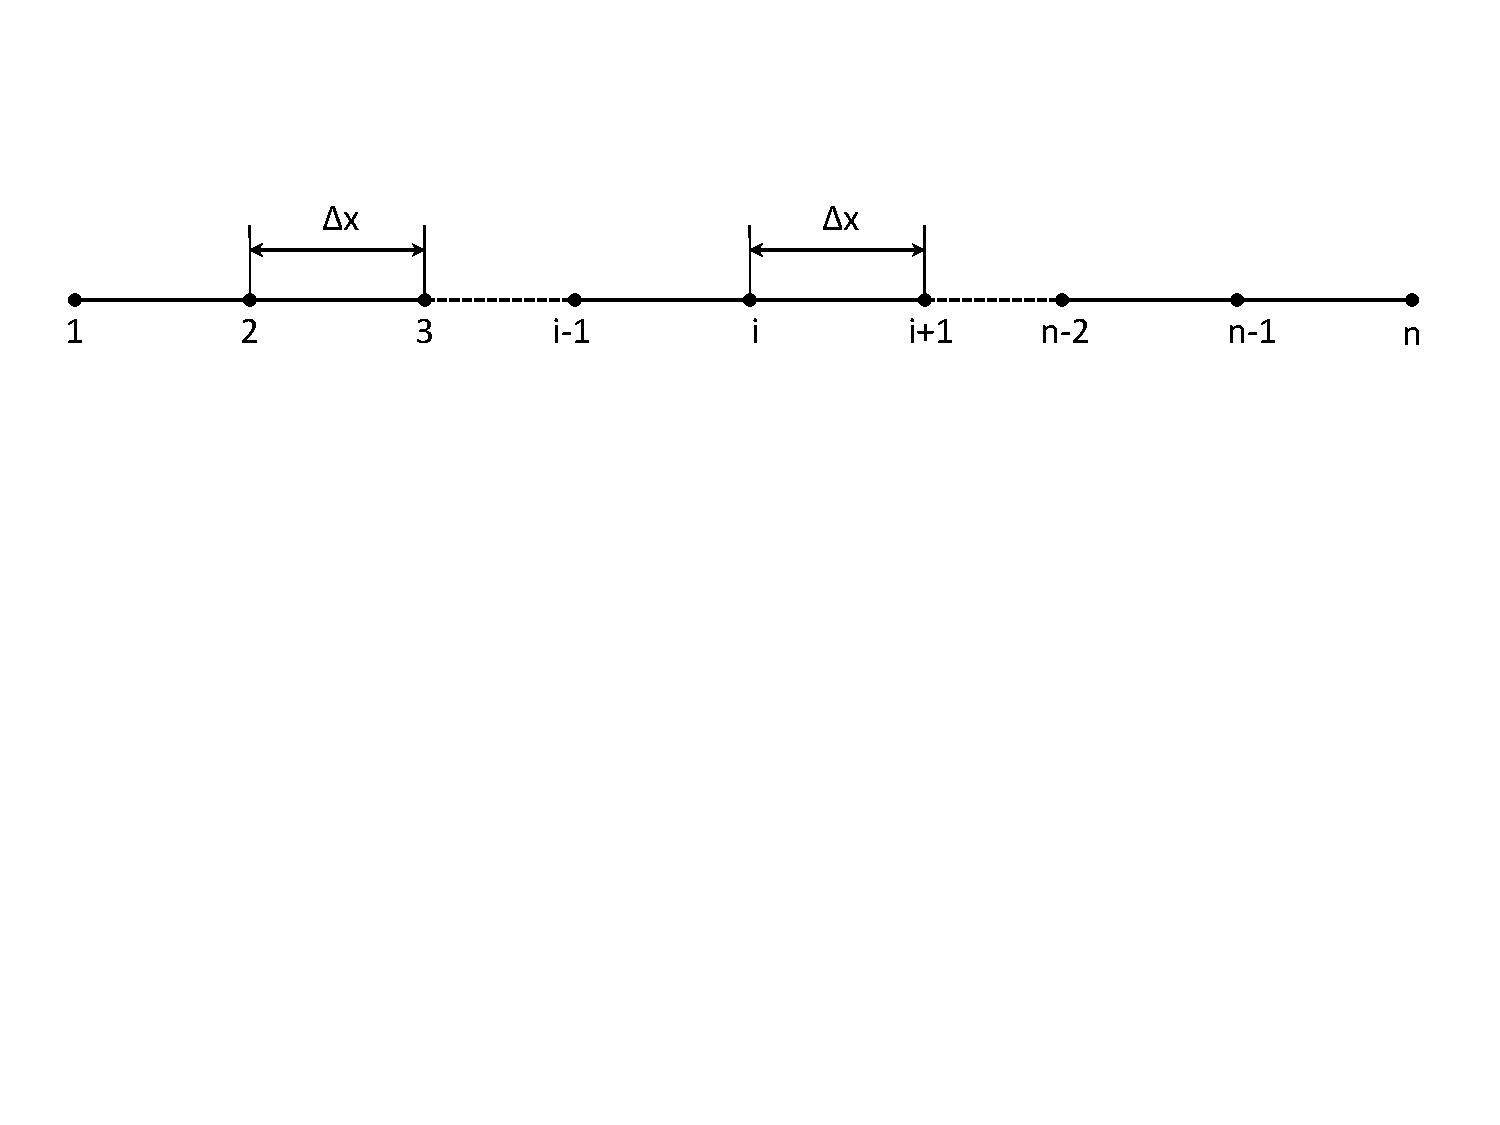
\includegraphics[width=11.5cm, height=1.5cm, clip]{./Figs/SchetchFDM.pdf}
       \end{center}}

\end{frame}


%%%
%%% Slide
%%% 
\begin{frame}
 \frametitle{Finite Difference Method (FDM)} 

\begin{enumerate}
   \setcounter{enumi}{4}
  \item <1-> Thus, the diffusion term can be redefined as,
     \visible<1->{
     \begin{equation}
         \Gamma\left(\frac{d^{2}\phi}{dx^{2}}\right)_{2}=\Gamma\frac{\phi_{i-1}+\phi_{i+1}-2\phi_{i}}{\left(\Delta x\right)^{2}}
     \end{equation}}
  \item <2-> And the source term can be evaluated at point $i$, i.e., $\mathcal{S}_{i}=\mathcal{S}\left(\phi_{i}\right)$. Thus the discrete form of Eqn~\ref{eq:1Dtransport_simplified} is,
     \visible<2->{
     \begin{equation}
         \Gamma\frac{\partial^{2}\phi}{\partial x^{2}} +\mathcal{S} = \Gamma\frac{\phi_{i-1}+\phi_{i+1}-2\phi_{i}}{\left(\Delta x\right)^{2}} + \mathcal{S}\left(\phi_{i}\right)
     \end{equation} }
  \item <3-> Here, we have a system of algebraic equations (for each point of the mesh) that can determine discrete values for $\phi$;
  \item <4-> The resulting system of equations can be solved by any (direct or iterative) method;
  \item <5-> The FDM is not inherently conservative, and can only be used in very simple geometries as it relies on structured mesh.

\end{enumerate}  
 
\end{frame}

%%%
%%% Slide
%%% 
\begin{frame}
 \frametitle{Finite Element Method (FEM)} 

\begin{enumerate}
  \item <1-> \textcolor{blue}{FEM} is a family of methods based on the minimisation of a weighted residual;
  \item <2-> The most 'popular' member of this $\lq$family' is the \textcolor{blue}{\it Galerkin FEM};
  \item <3-> Thus, let's assume that $\overline{\phi}$ is an approximation to $\phi$ of the solution of Eqn.~\ref{eq:1Dtransport_simplified};
  \item <4-> As $\overline{\phi}$ is just an approximation, i.e., it {\bf does not satisfy} Eqn.~\ref{eq:1Dtransport_simplified} {\bf exactly}, leading to a residual \textcolor{blue}{$\mathcal{R}$},
    \visible<4->{
      \begin{equation}
         \Gamma\frac{d^{2}\overline{\phi}}{dx^{2}} + \mathcal{S} = \mathcal{R}\label{eq:1Dtransport_simplified_FEM}
      \end{equation}}

  \item<5-> Thus, we aim to find $\overline{\phi}$ (over the domain $\Omega$) such that,
    \visible<5->{
      \begin{equation}
         \int\limits_{\Omega}\mathcal{W}_{i}\mathcal{R}dx = 0\;\;\; \forall i\in\left\{1, 2, ..., N\right\}\label{eq:1Dtransport_simplified_FEM_Residual}
      \end{equation}
    where $\mathcal{W}_{i}$ is a family of discrete weight function (over the number of grid points). The solution of Eqn.~\ref{eq:1Dtransport_simplified} requires that \textcolor{red}{$\mathcal{R}\rightarrow 0$} (Eqn.~\ref{eq:1Dtransport_simplified_FEM_Residual});}

     \visible<1->{ 
       \begin{center}
         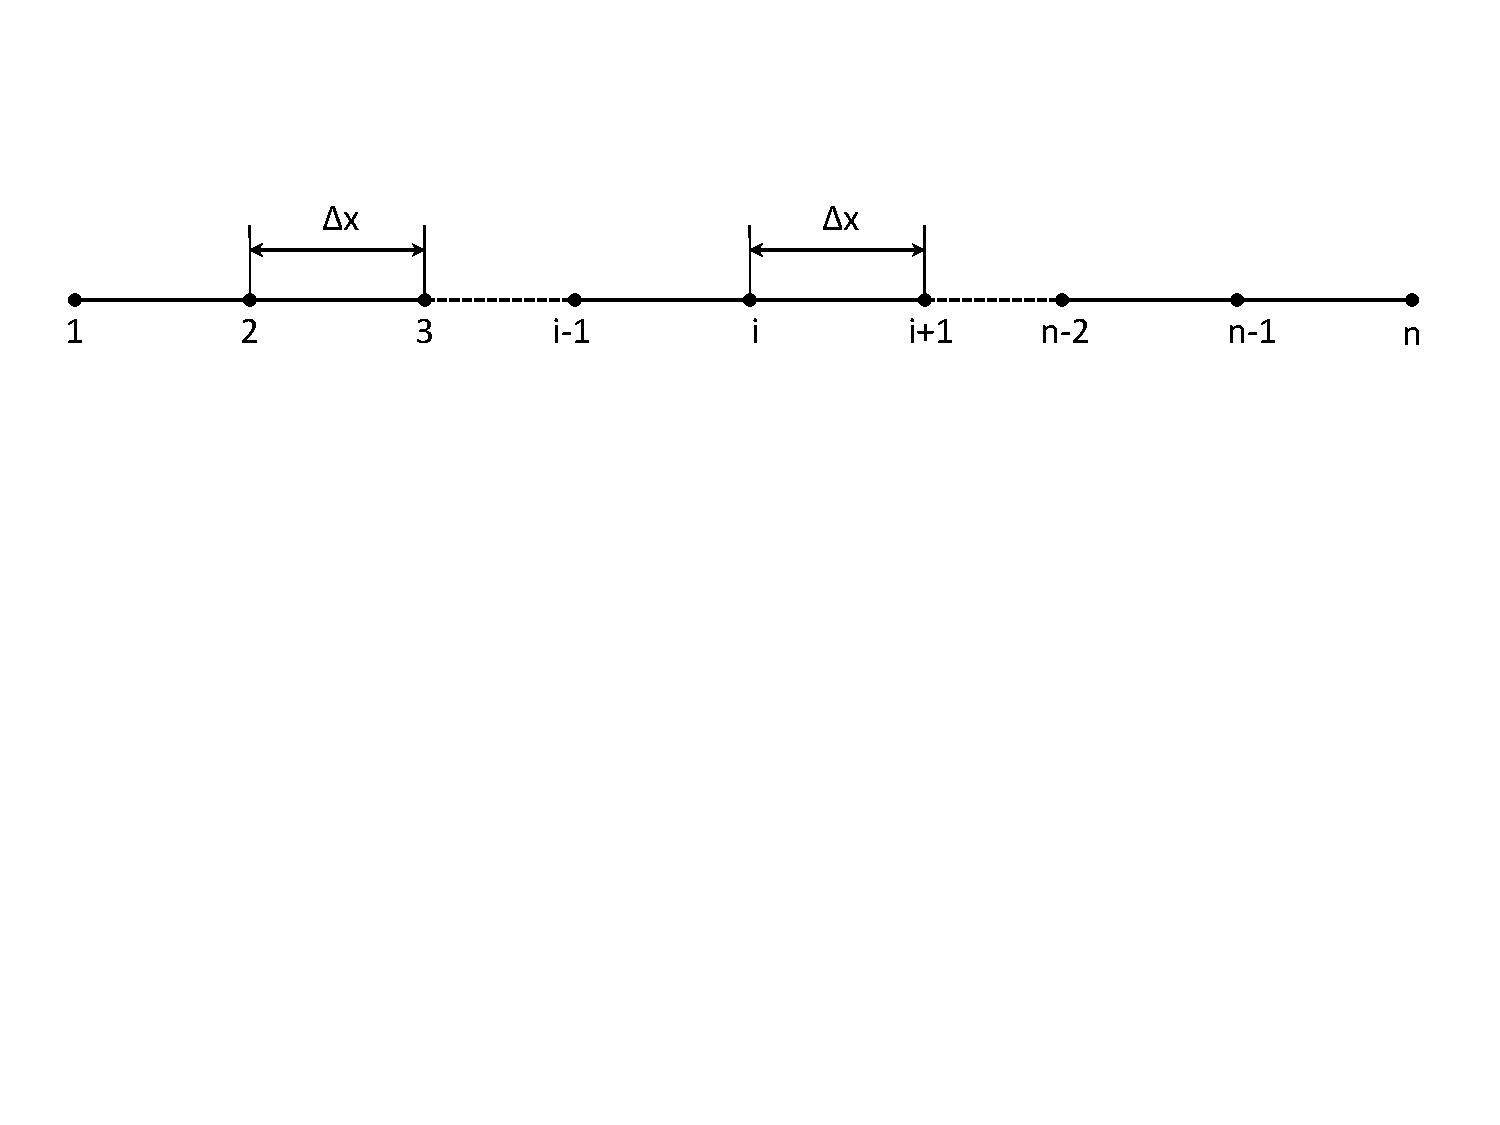
\includegraphics[width=11.5cm, height=1.5cm, clip]{./Figs/SchetchFDM.pdf}
       \end{center}}
   
\end{enumerate}  
 
\end{frame}

 
%%%
%%% Slide
%%% 
\begin{frame}
 \frametitle{Finite Element Method (FEM)} 

\begin{enumerate}
   \setcounter{enumi}{5}
     \item <1-> The \textcolor{blue}{weight functions $\left(\mathcal{W}_{i}\right)$} are local, i.e., they are {\it non-zero} at element $i$ and zero elsewhere;
     \item <2-> Local \textcolor{blue}{\it Shape Functions} for $\overline{\phi}$ are also introduced, i.e., $\overline{\phi}$ varies between nodes with a polynomial function;
     \item <3-> Applying \textcolor{blue}{weight and shape functions} into the integral (Eqn.~\ref{eq:1Dtransport_simplified_FEM_Residual}) results in a system of algebraic equations in the nodal value of $\phi$ that can be solved by a number of iterative methods;
     \item <4-> The \textcolor{blue}{Galerkin FEM} assumes that the residual is minimum (or equal to zero in a weighted sense) and therefore \textcolor{red}{{\bf conservation is not naturally enforced}}.

\end{enumerate}  
     \visible<1->{ 
       \begin{center}
         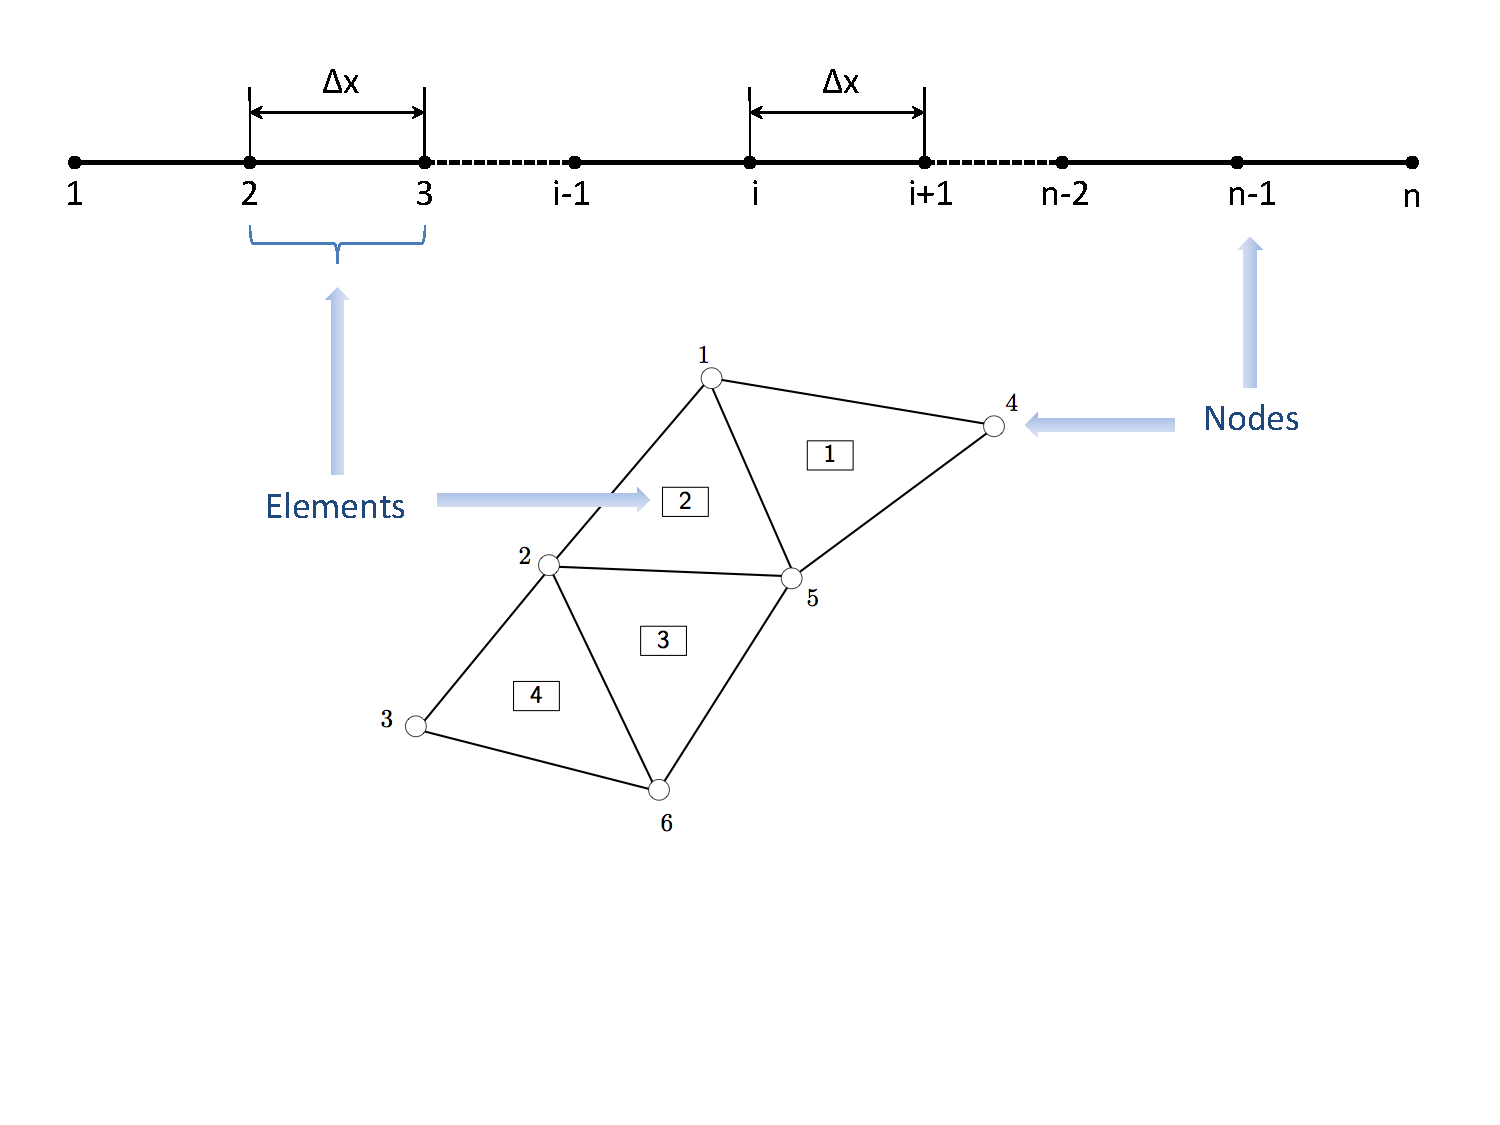
\includegraphics[width=7.5cm, height=3.5cm, clip]{./Figs/SchetchFEM.pdf}
       \end{center}}
 
\end{frame}


%%%
%%% Slide
%%% 
\begin{frame}
 \frametitle{Finite Volume Method (FVM)} 

\begin{enumerate}
     \item <1-> In the \textcolor{blue}{FVM}, the domain is discretised in a finite number of cells (also called \textcolor{blue}{control volumes}) over which the $\lq$quantity' $\phi$ is \textcolor{red}{\bf enforced} in a cell-averaged sense;
     \item <2-> Equation~\ref{eq:1Dtransport_simplified} is integrated over each cell; 
     \item <3-> The discrete values of $\phi$ are {\bf allocated} in the cell centroid ({\it W}, {\it P} and {\it E}) with faces denoted by {\it w} and {\it e}. The cell associated with {\it P},
       \visible<3->{ 
          \begin{equation}
            \int\limits_{w}^{e}\frac{d}{d x}\left(\Gamma \frac{d\phi}{d x }\right) dx + \int\limits_{w}^{e}\mathcal{S}dx = 0 \;\Longrightarrow \left(\Gamma\frac{d\phi}{d x}\right)_{e} - \left(\Gamma\frac{d\phi}{d x}\right)_{w} + \int\limits_{w}^{e}\mathcal{S}dx = 0
          \end{equation}}
\end{enumerate}  
     \visible<1->{ 
       \begin{center}
         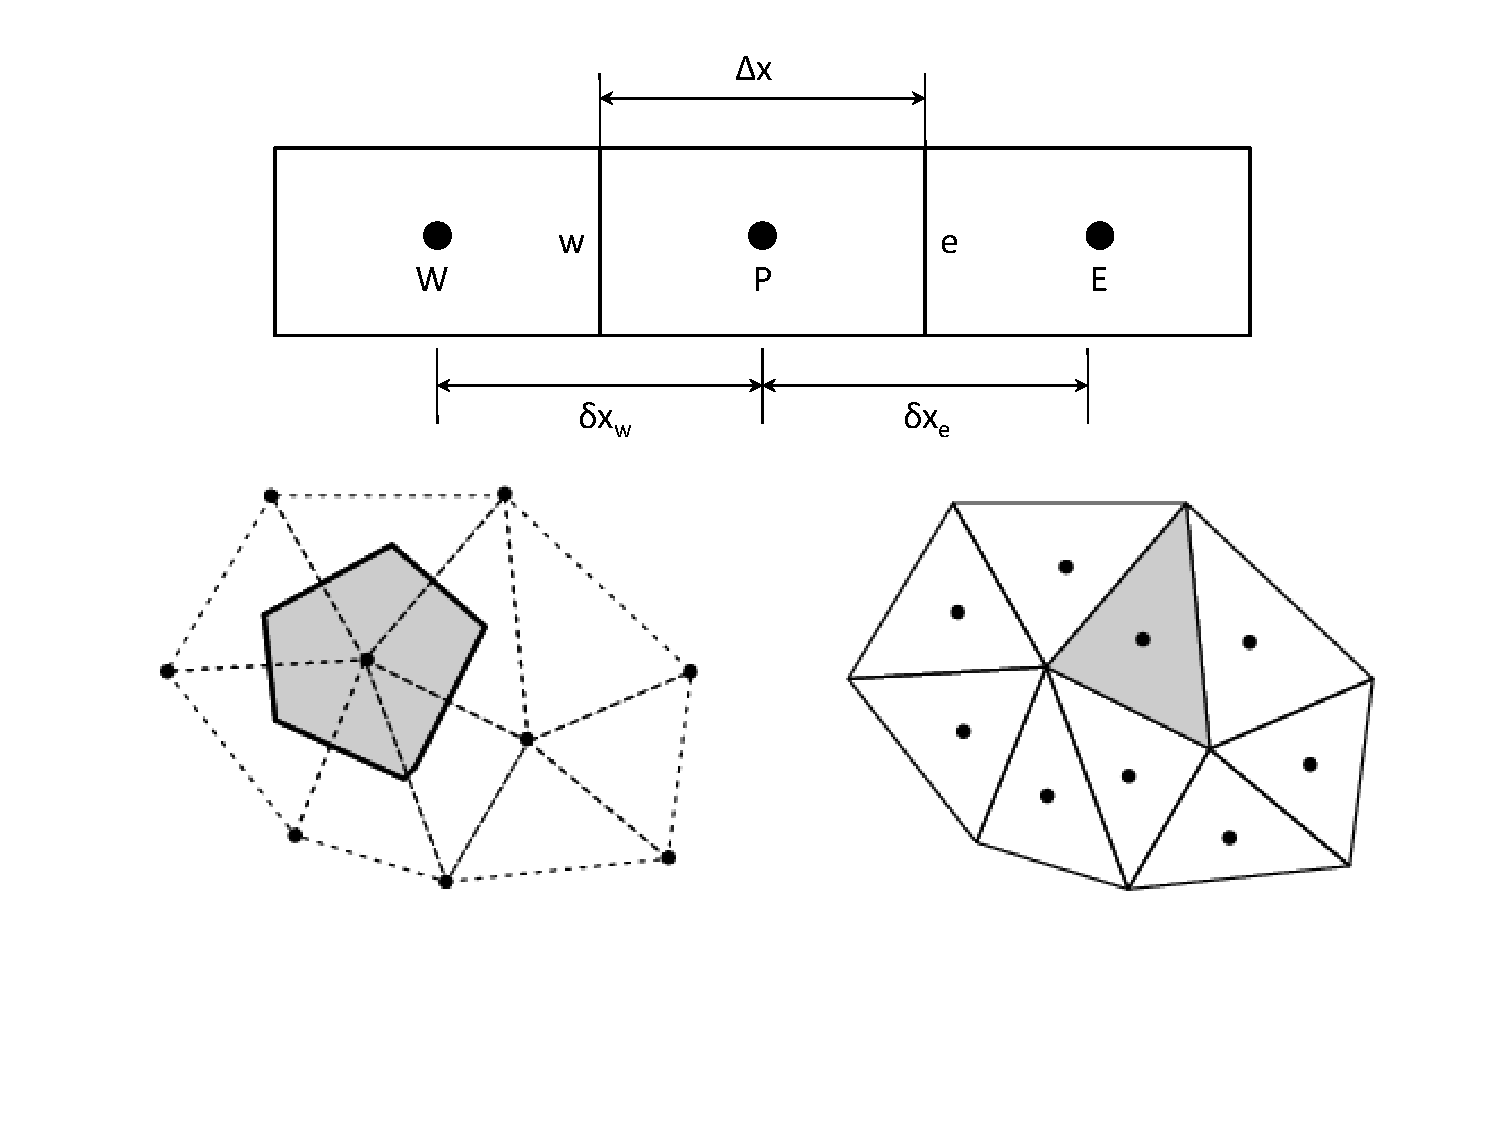
\includegraphics[width=4.5cm, height=3.5cm, clip]{./Figs/SchetchFVM2.pdf}
       \end{center}}
 
\end{frame}

%%%
%%% Slide
%%% 
\begin{frame}
 \frametitle{Finite Volume Method (FVM)} 

\begin{enumerate}
   \setcounter{enumi}{3}
     \item <1-> Now, if assume that $\phi$ varies linearly between cell centroids,
       \visible<1->{ 
          \begin{equation}
             \frac{\Gamma_{e}\left(\phi_{E}-\phi_{P}\right)}{\delta x_{e}} - \frac{\Gamma_{w}\left(\phi_{P}-\phi_{W}\right)}{\delta x_{w}} + \overline{\mathcal{S}}\Delta x = 0 \label{eq:fvmformulation}
          \end{equation}
       where $\overline{\mathcal{S}}$ is the average value of $\mathcal{S}$ over the cell.}
     \item <2-> Equation~\ref{eq:fvmformulation} can be rewriten as
       \visible<2->{ 
          \begin{equation}
             \alpha_{P}\phi_{P} = \alpha_{E}\phi_{E}+\alpha_{W}\phi_{W}+\beta \label{eq:fvmformulation2}
          \end{equation}
       where $\alpha_{i}=\Gamma_{i}/\delta x_{i}$ (for $i=W, E$), $\alpha_{P} = \alpha_{E}+\alpha_{W}$ and $\beta=\overline{\mathcal{S}}\Delta x$.}
     \item <3-> Equation~\ref{eq:fvmformulation2} can be applied to all cells in the domain resulting in a system of algebraic equations that can be solved by any iterative method;
      
\end{enumerate}  
     \visible<1->{ 
       \begin{center} 
         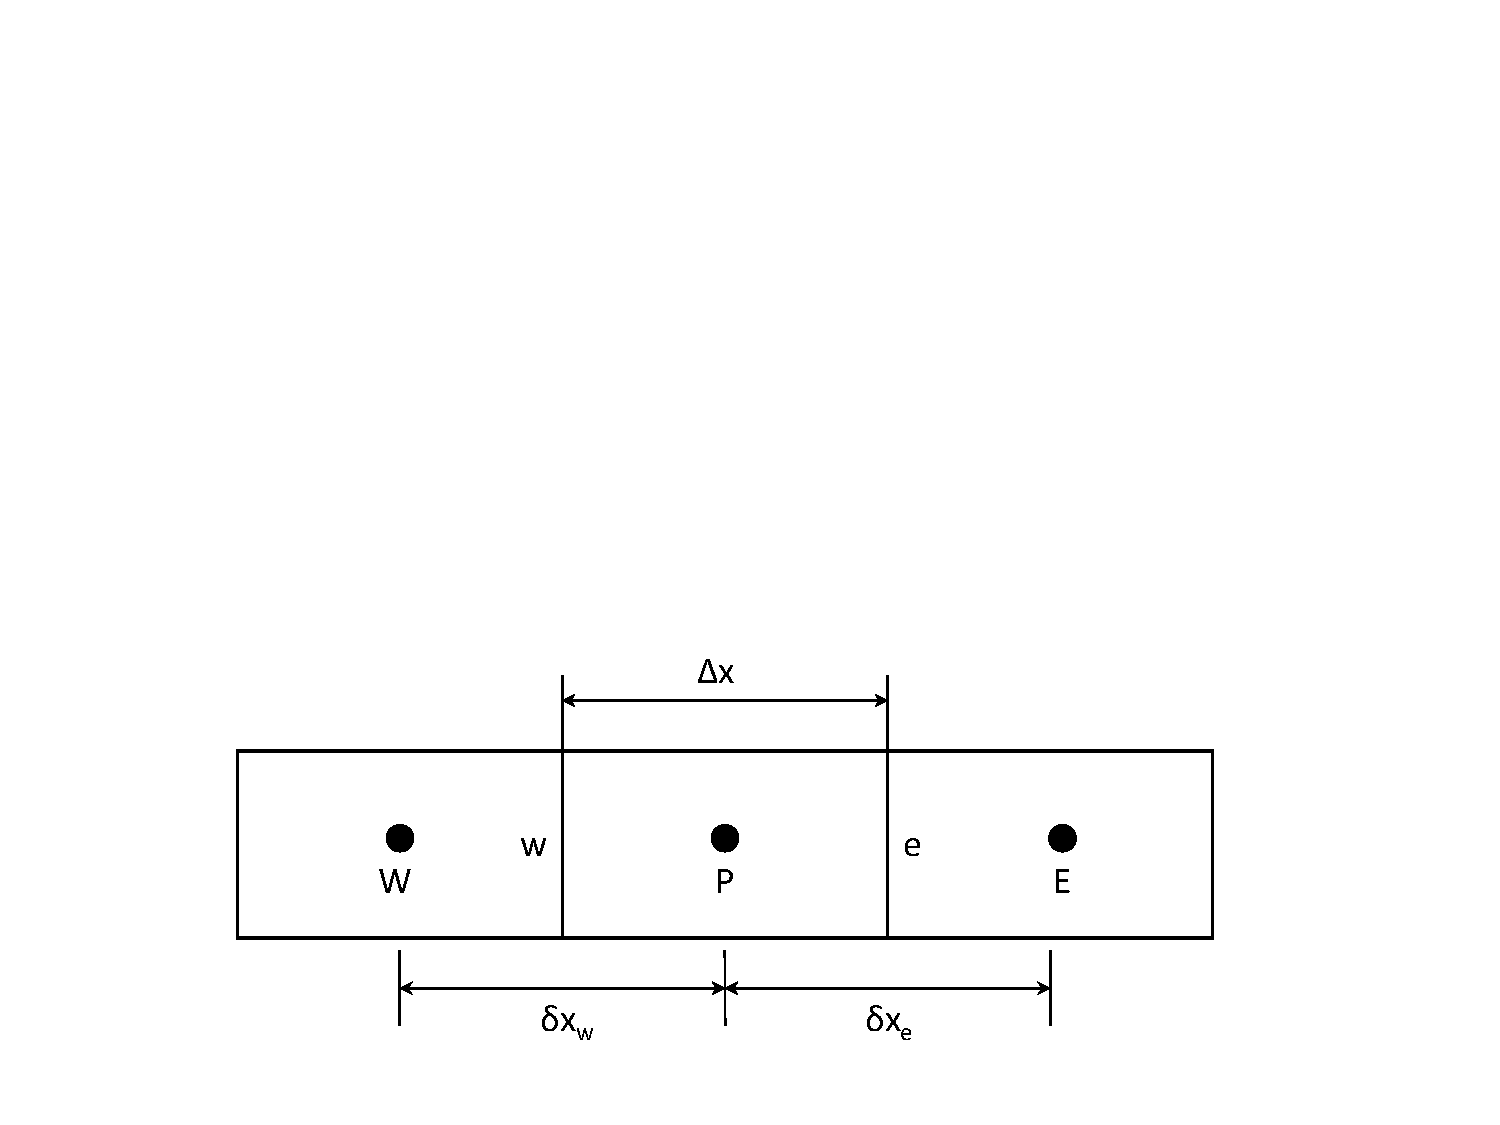
\includegraphics[width=8.5cm, height=2.5cm, clip]{./Figs/SchetchFVM.pdf}
       \end{center}}
 
\end{frame}

\begin{comment}
%%%
%%% Slide
%%% 
\begin{frame}
 \frametitle{Finite Volume Method (FVM)} 

\begin{enumerate}
   \setcounter{enumi}{6}
     \item <1-> Now, if assume that $\phi$ varies linearly between cell centroids,
       \visible<1->{ 
          \begin{equation}
             \frac{\Gamma_{e}\left(\phi_{E}-\phi_{P}\right)}{\delta x_{e}} - \frac{\Gamma_{w}\left(\phi_{P}-\phi_{W}\right)}{\delta x_{w}} + \overline{\mathcal{S}}\Delta x = 0 \label{eq:fvmformulation}
          \end{equation}
       where $\overline{\mathcal{S}}$ is the average value of $\mathcal{S}$ over the cell.}
     \item <2-> Equation~\ref{eq:fvmformulation} can be rewriten as
       \visible<2->{ 
          \begin{equation}
             \alpha_{P}\phi_{P} = \alpha_{E}\phi_{E}+\alpha_{W}\phi_{W}+\beta \label{eq:fvmformulation2}
          \end{equation}
       where $\alpha_{i}=\Gamma_{i}/\delta x_{i}$ (for $i=W, E$), $\alpha_{P} = \alpha_{E}+\alpha_{W}$ and $\beta=\overline{\mathcal{S}}\Delta x$.}
     \item <3-> Equation~\ref{eq:fvmformulation2} can be applied to all cells in the domain resulting in a system of algebraic equations that can be solved by any iterative method;
      
\end{enumerate}  
     \visible<1->{ 
       \begin{center} 
         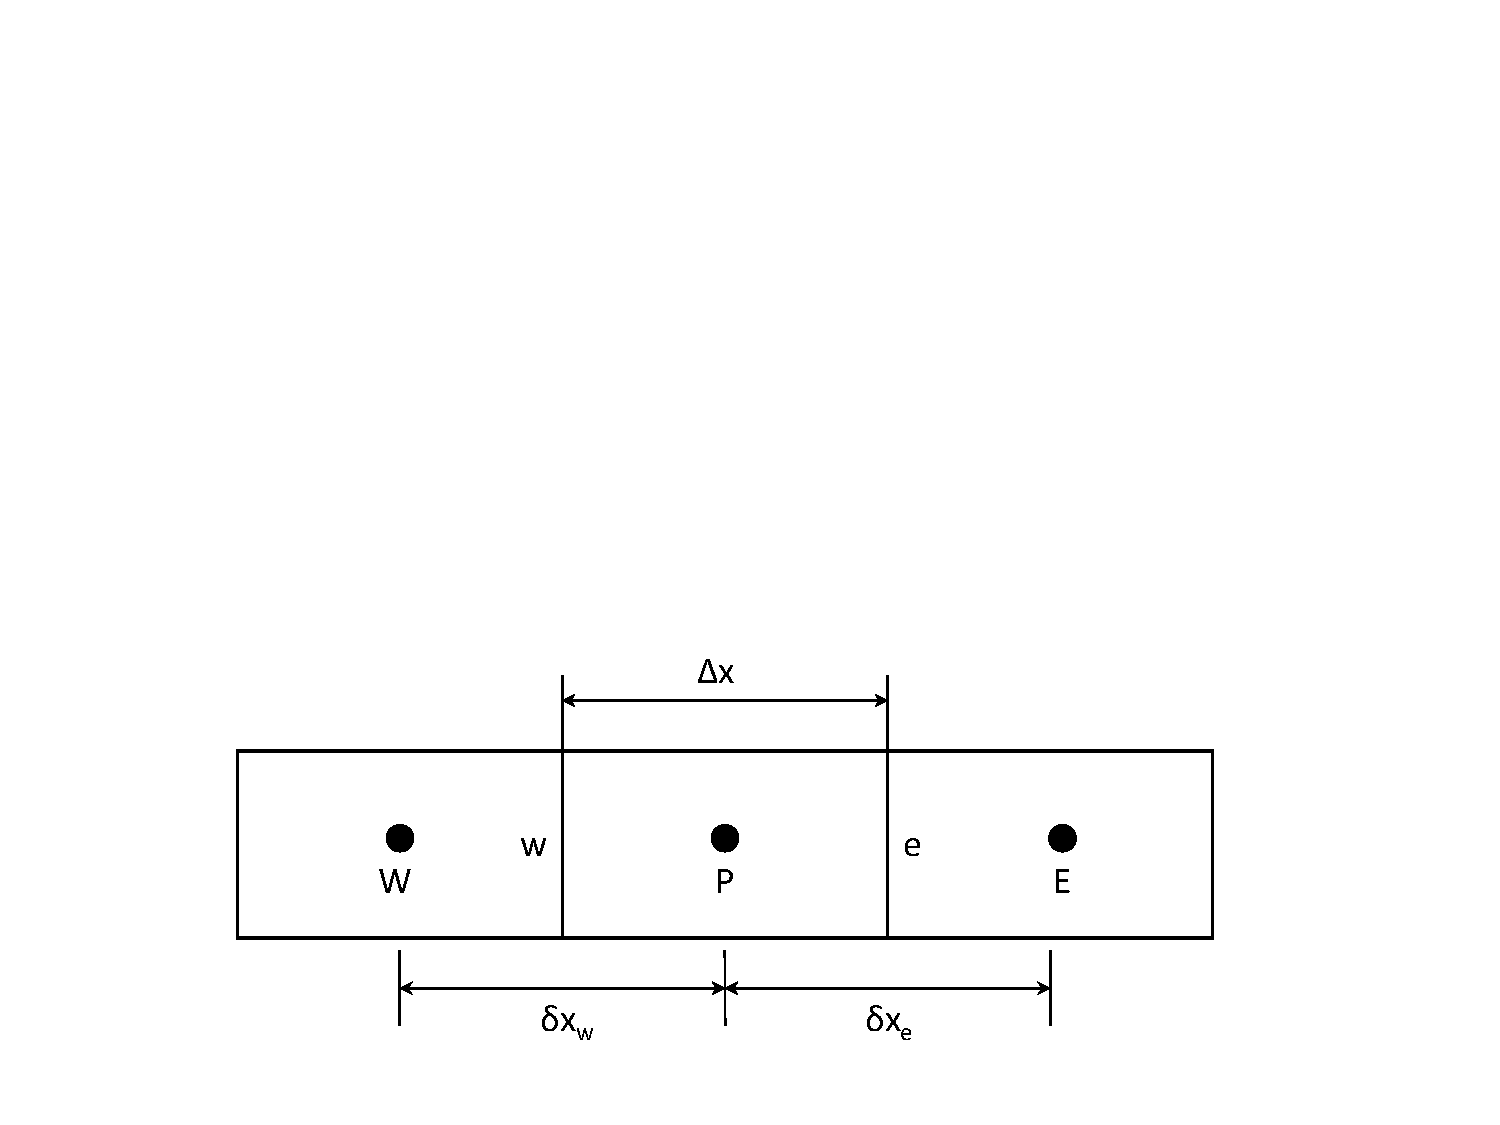
\includegraphics[width=8.5cm, height=2.5cm, clip]{./Figs/SchetchFVM.pdf}
       \end{center}}
 
\end{frame}
\end{comment}
 
\end{document}
